%methods

\subsection{Overview}

Figure \ref{fig1} provides an overview of the 
developed computational pipeline. 
%
We obtain 16S metagenomic sequence reads from patients who 
had encephalopathy and liver cirrhosis, no encephalopathy but liver cirrhosis, and controls (with neither phenotype). The input sequence 
reads are annotated using a taxonomic profiling approach (Kraken) or 
an unsupervised binning approach (UCLUST). The output of this annotation phase 
features are generated, which are passed on the binary support vector machine 
classifier (SVMs).  We used the  svm-light implementation \cite{Joachims08}  
to perform the classification of whether or not a patient 
had a clinical phenotype. We compared the classification performance of the 
SVM classifier with the two intermediate sequence representations obtained from 
UCLUST and Kraken. We also applied feature scaling and 
selection techniques to improve the classification results.

\begin{figure*}[t]
\begin{center}
\caption{Pipeline Overview. \label{fig1}}
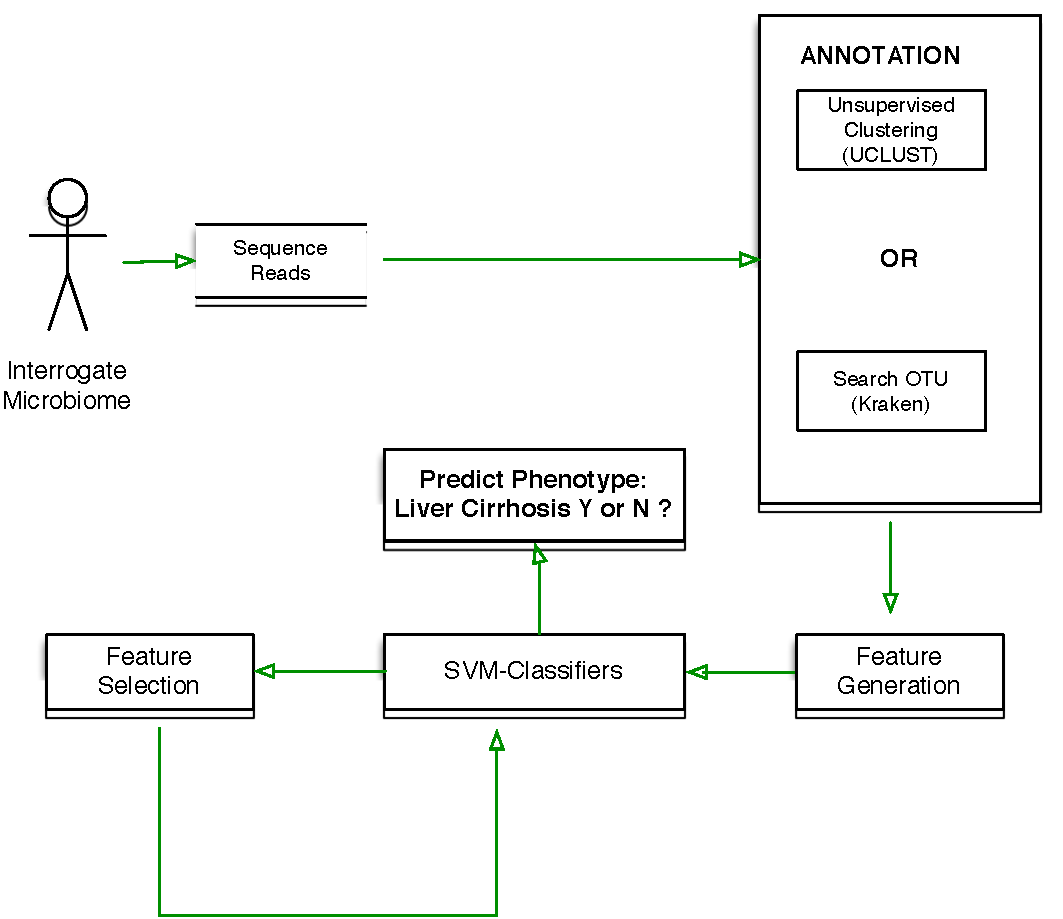
\includegraphics[scale=0.7]{./diagrams/concept}
\end{center}
\end{figure*}

\subsection{Unsupervised Clustering using UCLUST}
\label{uclustmethods}

In this work we evaluate the use of an unsupervised approach 
for representing our input metagenome sequence reads. Specifically, we 
  use UCLUST \cite{edgar2010search} due to its superior performance in terms 
  of run time and accuracy.
%
%
%
UCLUST \cite{edgar2010search} follows a greedy, iterative clustering approach. As a first 
step, this approach identifies exact matches of fixed length between sequence pairs known 
as seeds. These seeds are then extended by allowing for a few mismatches and/or gaps between 
the aligned pairs. Seeds scoring above a certain threshold are chosen as high segment pairs (HSPs)  and 
used for further processing. As such, the step eliminates a lot of pairwise comparisons. 

Then UCLUST follows an 
incremental approach for assigning the input sequences to the different bins. 
%
%
The clustering solution is initialized as an empty list. Sequences are then 
incrementally added to the clusters existing within the list. 
%
Each unassigned input sequence is compared to the cluster representatives within the list using 
the fast indexing search technique that uses the HSPs. If a match is found with one of the 
cluster representatives, then that sequence is assigned to that particular cluster or the 
input sequence forms a new cluster. 
%
UCLUST ensures
that the cluster representatives are sequences with the largest length. 

\subsection{Supervised Taxonomic Identification using Kraken}

We also evaluate the use of a search based 
approach to taxonomically label our sequence reads. We use 
Kraken for this, due to its strong performance in terms of run time 
and precision. Kraken finds $k$-mers in an input 
sequence read and queries a database of OTUs. It then associates the 
read with the lowest common ancestor (LCA) of the genomes that contains $k$-mers from the read \cite{Kraken}. In order to reduce 
the number of false positives, Kraken does not classify reads for 
which it does not find sufficient evidence of any match.


This approach is designed to perform quickly and with 
high precision. However, it also involves downloading and building 
a large database to query. It is often infeasible to download and 
build the database in its entirety, so a smaller custom  
subset of the database is available for testing 
purposes. We used this 
subset of the entire database in this study (referred to as kraken-light).


\subsection{Classification using Support Vector Machines (SVMs)}

Support Vector Machines (SVMs) \cite{vap95} are 
one of the most powerful and versatile binary classifiers used 
in myriad applications. 
%
For a  binary classification problem, the support 
vector machine (SVM) \cite{vap95} framework 
maximizes the separation between the two classes.
%

Given an input set of positive training instances and 
negative training instances, the SVM classifier learns a 
mathematical function $f$  that maximizes the separation between 
the given positive and negative training instances. The function $f$ will then be able to predict whether a new instance (considered a test instance) should have a positive or negative class label.
%
For our formulation we use SVMs to make clinical phenotype prediction for each 
patient sample 
based on their  input metagenome sequence samples represented with their 
clustering or taxa membership features. 

For all the available microbiome samples,  we have a set of reads processed via UCLUST or Kraken. 
%
Each patient is associated with a vector that is used by the SVM to help build $f$. Each row in the vector, called a feature, corresponds to a certain species, and the value for that row corresponds to how closely the read from the patient matched what the species was expected to look like. The exact process of assembling a feature vector for a 
patient depends on which data representation is being used. For 
UCLUST, we use each cluster seed 
as a feature. For each input 
sequence, we use the percentage match to its cluster seed as 
the value for that feature and average the 
sequence match if multiple reads from the metagenome samples 
are assigned to the same cluster by UCLUST. 
%
For Kraken, we use the taxonomic label associated 
with the read as the feature for the SVM. The percentage match of the 
read to that label is used as the feature value. Similar 
to UCLUST, we average the similarity score if multiple reads align to the 
same taxonomic class label. 
%
Our feature selection process involves discarding Kraken's unlabeled 
reads and UCLUST's clusters with only one read (singletons). 

We used cross-validation and a held out set procedure (discussed in the next 
Section) to assess the performance of SVM classification using UCLUST and Kraken
as intermediate representations.


